\chapter{\K{}-based Computer Interpretable Guidelines}

In \autoref{chapter:separating-concerns}, we described an
architecture for building safe and modular clinical decision support systems.
We split \CDSSs{} into three separate components:
\begin{enumerate*}[label=(\alph*)]
  \item a frontend that facilitates interaction with \HCPs{},
  \item a backend that serves as a computer-interpretable encoding of the \BPG{}, and,
  \item additional infrastructure that wires components together.
\end{enumerate*}
This, and upcoming chapters, focus on building backends for \CDSSs{}
utilizing the \emph{semantics-first} approach described in
\autoref{chapter:semantics-first-cdss}. By semantics-first, we
mean that:
\begin{enumerate*}[label=(\alph*)]
 \item the semantics of medical knowledge in the \BPG{} is
 accurately captured, and,
 \item the semantics of the language used to describe the
 \BPG{} is formally defined.
\end{enumerate*}

In \autoref{sec:generic-bpg}, we briefly described characteristics
of \BPGs{} that a \CIG{} language must accommodate.
To this end, we attempted to come up with a framework that
can accommodate expressing a large number of diverse \BPGs{}.
Thus, we broke \BPGs{} into smaller statements that we organized
into:
\begin{itemize}
  \item a workflow containing statements that are executed sequentially, and,
  \item workflows within a guideline may be executed concurrently.
\end{itemize}

In this chapter, we describe a methodology to encode real-world \BPGs{}
as $\K$ definitions. Execution in $\K{}$ is inherently concurrent---
if more than one $\K{}$ rule can apply, then $\K$ non-deterministically
chooses one. Thus, we describe a way of systematically encoding
medical knowledge in \BPGs{} as $\K$ definitions. First, in
\autoref{sec:acls}, we introduce a real world \BPG{} that will be
utilized as running-example in the rest of this chapter. Note that
we intentionally choose real-word examples, instead of small toy cases,
to highlight that our philosophy scales to work in the real-world.
Next, \autoref{sec:kacls-cdss} describes $\KACLS{}$, a $\K$-based tool
to assist \HCPs{} conform to \ACLS{} guidelines that attempts to
follow the \emph{semantics-first} approach. Specifically,
we come up with an abstract representation that captures the semantics
of the \BPG{} from \autoref{sec:acls} with enough details to
enable computer-interpretation. Finally, in \autoref{sec:kacls-backend},
we describe a way to embed said abstract representation into a concrete
$\K$ definition for execution.

\section{Advanced Cardiovascular Life Support Guidelines (\ACLS{})}\label{sec:acls}

\begin{figure}[t!]
  \centering
  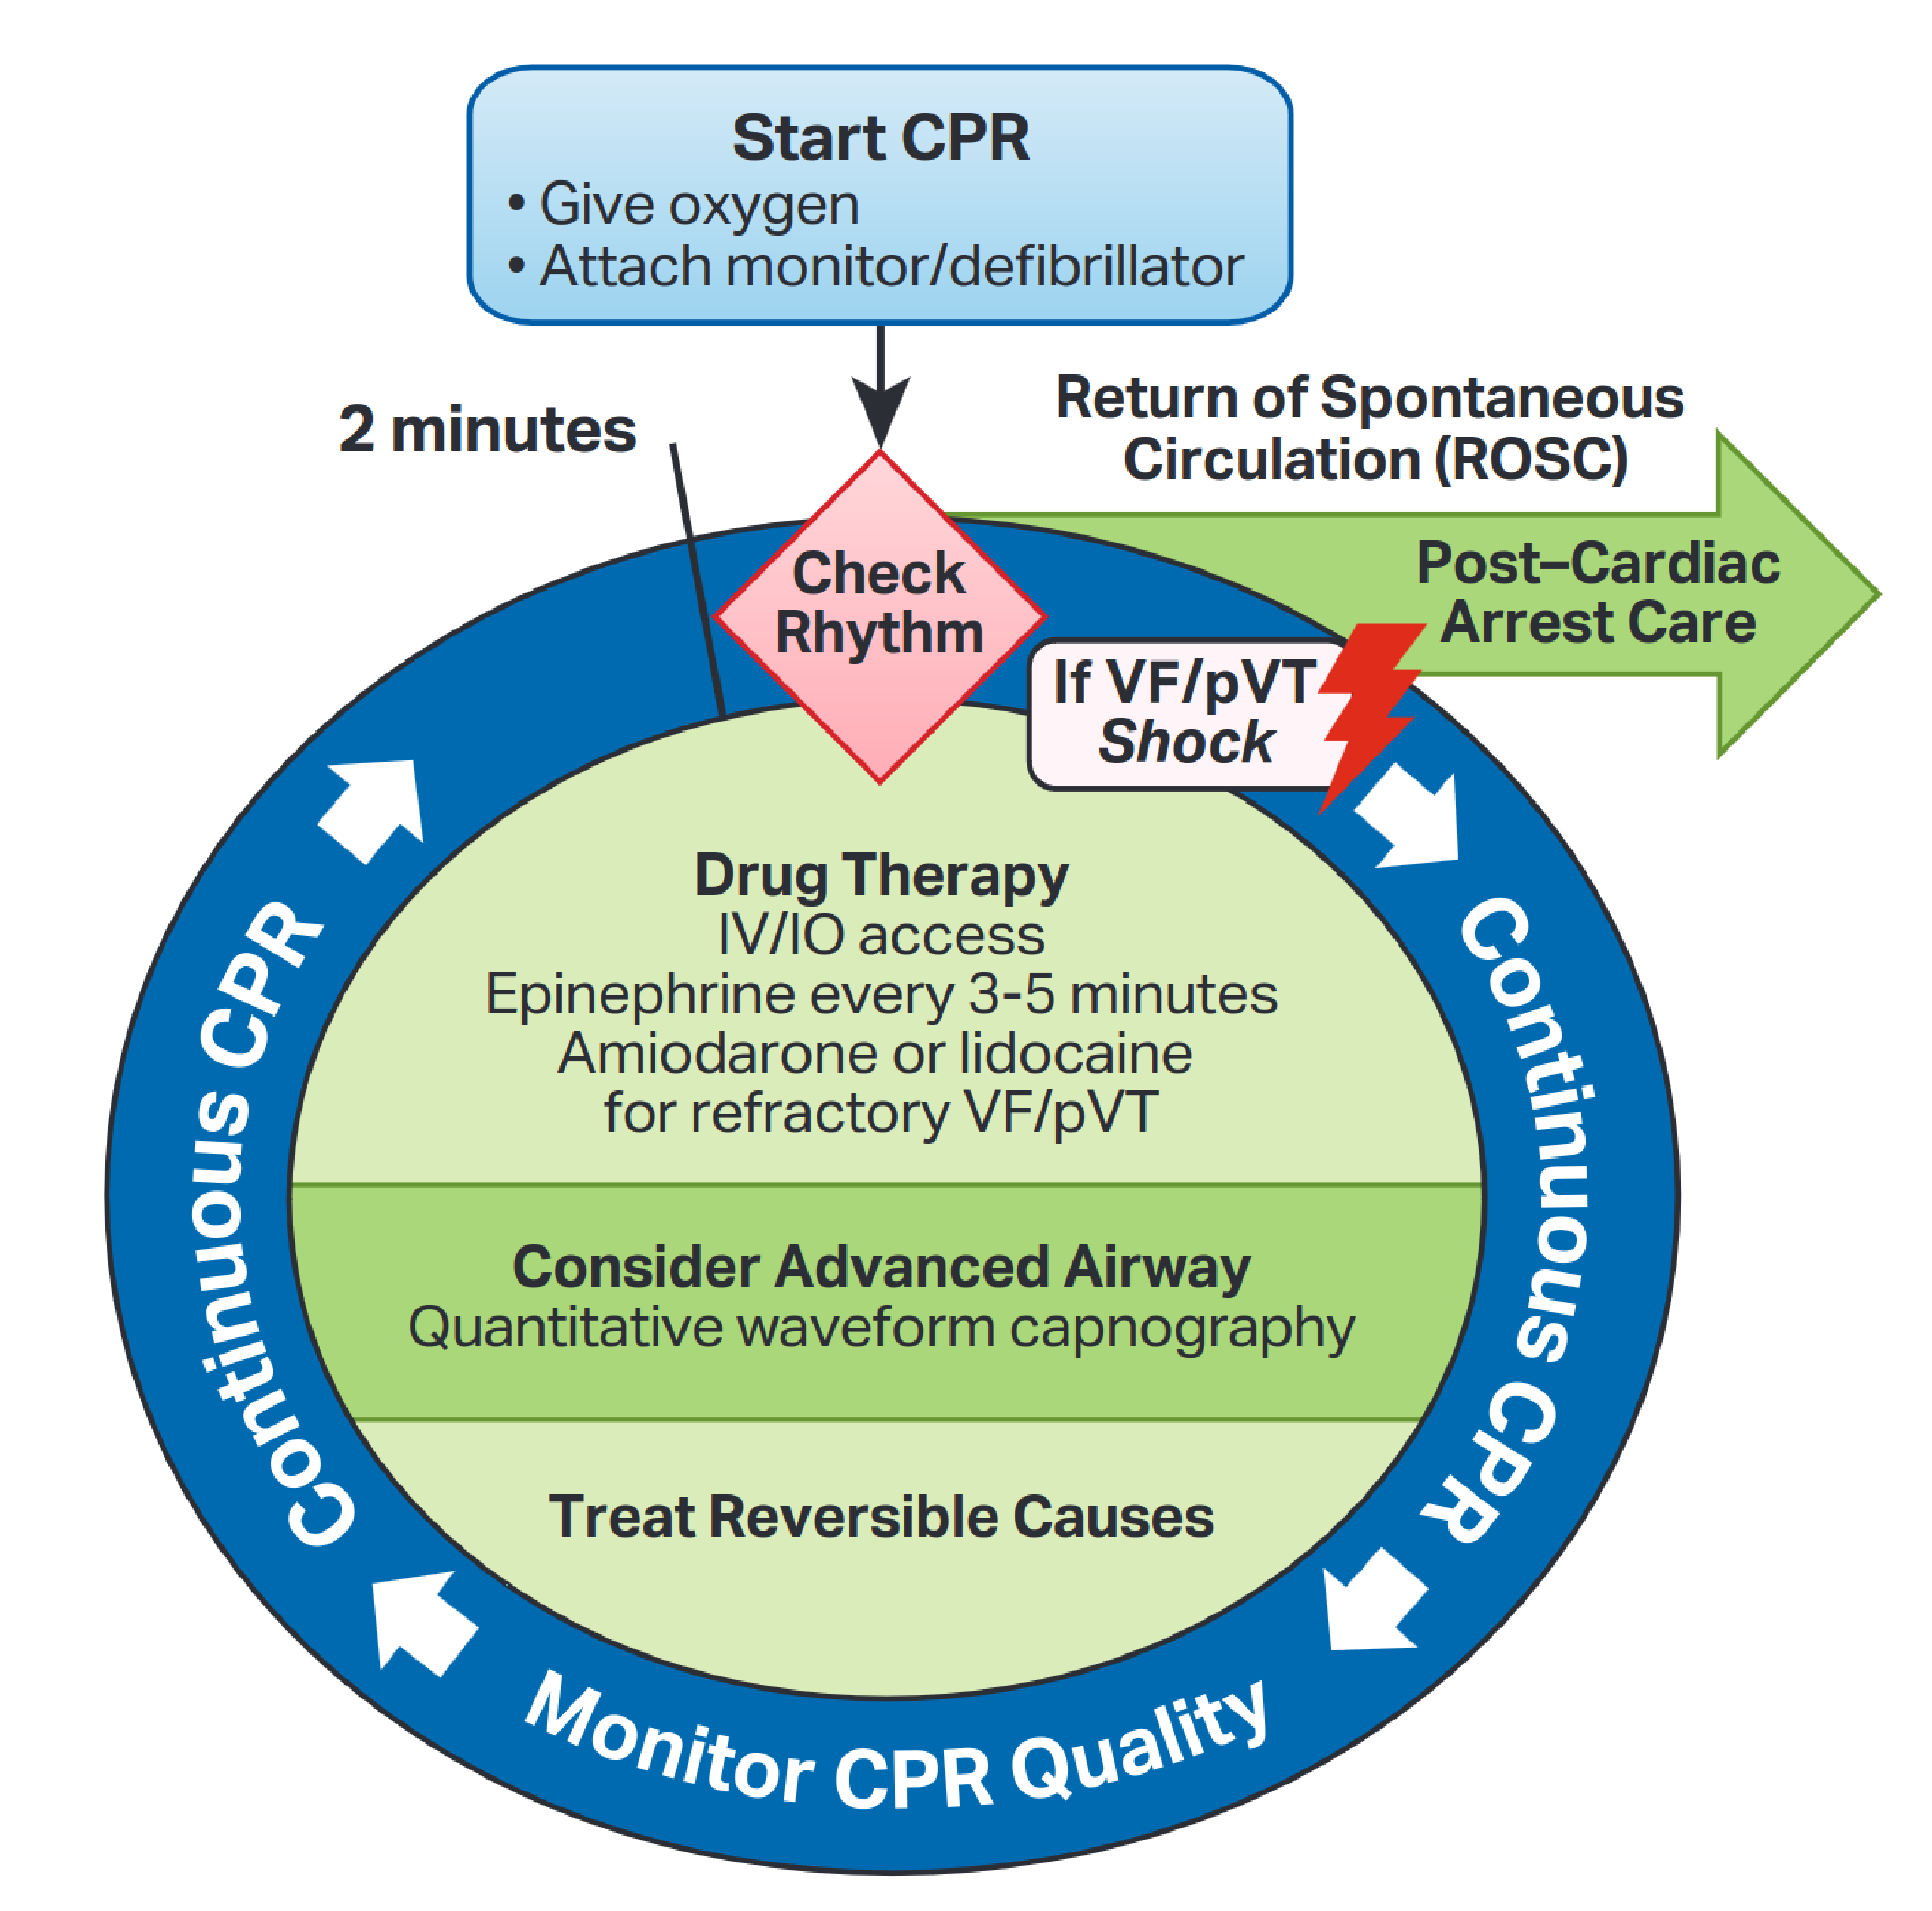
\includegraphics[width=0.6\textwidth]{acls-algorithm}
  \caption{Advanced Cardiac Life Support Guidelines}\label{fig:acls-algorithm}
\end{figure}

Advanced Cardiovascular Life Support (\ACLS{}) are a set of \BPGs{} periodically
published by the American Heart Association (\AHA{}) for management of
life-threatening cardiac conditions that will cause of have caused cardiac
arrest. The conditions that the guidelines treat range from dangerous arrhythmias, i.e.,
irregularities in heart's rhythm, to cardiac arrest.---a cardiac emergency where
the heart stop pumping \cite{ACLSWikiEntry}.
The guidelines, according to the AHA{}, \say{are based on the most current
and comprehensive review of resuscitation science, systems, protocols, and
education} \cite{ACLSUrl}.

\autoref{fig:acls-algorithm} shows the \AHA{}'s guidelines for advanced
life support (\ALS{}) for managing cardiac arrest in adults \cite{ACLSGuidelineUrl}.
\AHA{} publishes guidelines
for basic life support (\BLS{}), and pediatric counterparts of both. While
\BLS{} is meant for a first responder to provide treatment with
limited resources, such as an automatic emergency defibrillator (\AED{}),
\ACLS{} is supposed to be followed by teams of
trained professionals with advanced equipment for airway management,
drug delivery, etc.

\subsubsection{Why build \CDSSs{} for \ACLS{}?}

Cardiac arrest treatment is extremely time-critical, and outcomes
become significantly worse with every passing minute. This
gathering relevant data about the patient infeasible. Moreover, as
the seriousness of the condition necessitates multiple, simultaneous treatments
to be administered rapidly, intervention is usually executed following
standardized \ACLS{} algorithms \cite{ACLSWikiEntry}.

Prompt \ACLS{} guidelines-conformant treatment has been
shown to improve patient outcomes \cite{HonarmandResuscitation18}.
Moreover, deviations from the guidelines in in-hospital cases has been
associated with decreased rates of return of spontaneous circulation (\ROSC{}),
survival to discharge, and survival to discharge with favorable neurological
outcomes \cite{CrowleyResuscitation20}. Studies have also found that
inadequate \ACLS{} training can lead to poor retention, resulting
in reduced \ACLS{} conformance \cite{KiddJCN07}. Thus,
a \CDSS{} that can provide situation-specific guidance about
the next steps, especially in cases where \HCP{} training might be inadequate,
can potentially improve compliance, and consequently outcomes.

\subsubsection{A Brief Overview of Advance Life Support Guidelines for Cardiac Arrest:}

As we aren't concerned with intricacies of medical knowledge in the guideline,
we present a brief and simplified description of the guideline-prescribed treatment.
As \ALS{} is supposed to be performed in settings where necessary equipment is
available, a electrocardiogram (EKG) machine is utilized to
monitor the patient's cardiac rhythm. Certain cardiac arrhythmias, characterized
by cardiac rhythms referred to as \emph{shockable}, must be treated
by delivering a therapeutic electric shock
\cite{DefibrillationWikiEntry}. As shown in \autoref{fig:acls-algorithm},
treatment has several parallel workflows such as:
\begin{itemize}
  \item Periodic monitoring of the cardiac rhythm, and in case of a
    \emph{shockable} rhythm, using a defibrillator.
  \item Continuous cardiopulmonary resuscitation (\CPR{}).
  \item Administration of vital drugs such as
    epinephrine every few minutes.
\end{itemize}
As \autoref{fig:acls-algorithm} suggests, these workflows have to be
performed rapidly and periodically. As the duration of the intervention
is typically a few minutes, making optimal use of available time is critical to
outcomes.

\section{The \KACLS{} System}\label{sec:kacls-cdss}

\begin{figure}[t!]
  \centering
  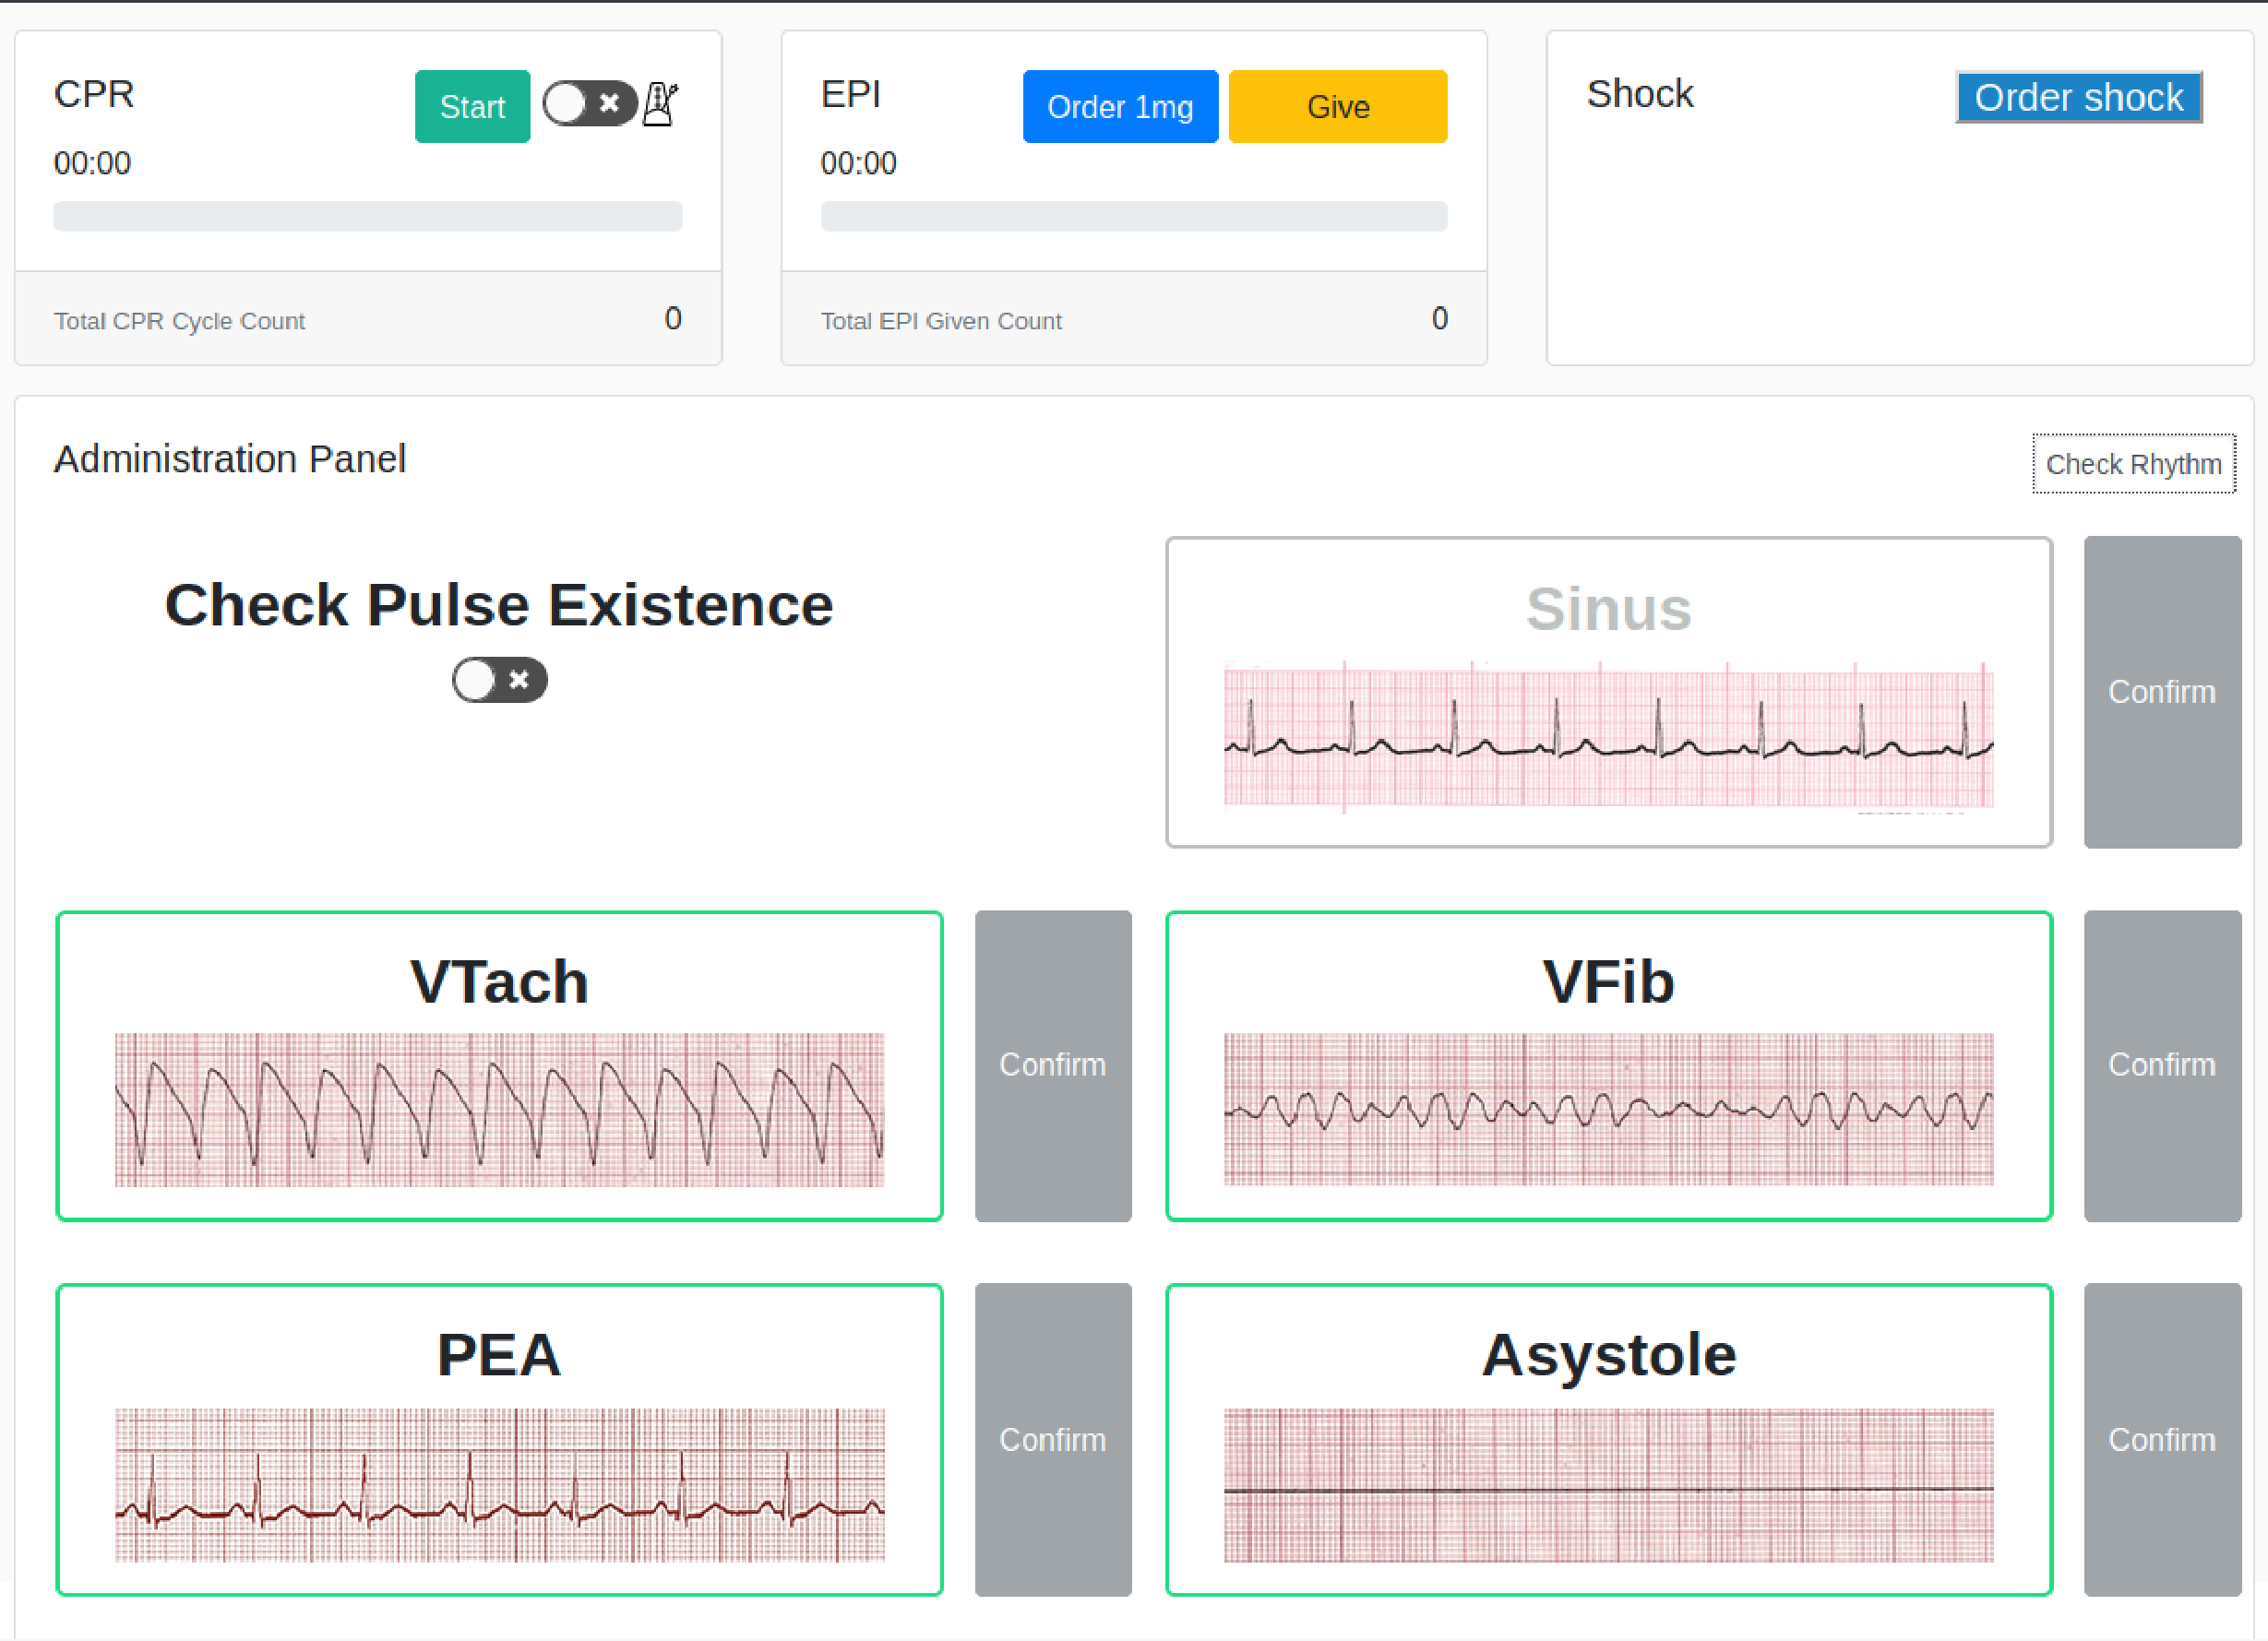
\includegraphics[width=0.65\textwidth]{acls-tool}
  \caption{Snapshot of \KACLS{}}\label{fig:kacls-snapshot}
\end{figure}

\autoref{fig:kacls-snapshot} shows a snapshot of our \CDSS{} for
enabling compliance to the advanced life support guidelines described in
\autoref{sec:acls}. Advanced life support is supposed to be performed by
a team of \HCPs{}, that take on roles such as a leader, \CPR{}-provider,
airway/respiratory specialist, Intravenous access (IV) and drug administration
specialist, pharmacist, defibrillator attendant and members that serve as
backups \cite{ACLSWikiEntry}. The leader is responsible for coordinating
treatment, our tool render support through a handheld tablet held by the leader.
\autoref{fig:kacls-snapshot} show a snapshot of said tablet's main screen.
Decision support, in the form of time-sensitive reminders, warnings when
procedures are stopped prematurely, or exceed stipulated limitations, and
confirmations regarding the patient rhythm's are provided on the screen
through popups and progress bars. For example, when the leader instructs
the team to start CPR, and presses the \say{Start} button under the \say{CPR}
section of the screen. A timer displays the duration and appropriate warnings
about prematurely stopping CPR, or exceeding the time for a \CPR{} cycle are
displayed.

In \autoref{sec:modular-cdss-architecture}, we described
conceptual components of \CDSSs{}, and argued in favor
of developing \CDSSs{} using independently developed and maintained codebases
aligned with these components. The \KACLS{} system follows
this philosophy, and has:
\begin{enumerate*}[label=(\roman*)]
  \item a simple \emph{frontend} written in Javascript using React \cite{ReactJSUrl} that handles
    user interaction, and,
  \item a $\K$-based HTTP server that encodes the \ACLS{} guideline
    and interacts with the frontend.
\end{enumerate*}
The use of the Javascript based frontend allows our application
to run on any modern web-browser. As shown in figure \ref{fig:kacls-snapshot},
our frontend consists of forms and buttons that correspond to procedures
in the algorithm in figure \ref{fig:acls-algorithm}. For example, the
\say{Start} button in the CPR box results in a two minute timer corresponding
to the \say{2 minute continuous CPR} procedure in the informal description.
The frontend is simple and doesn't contain any guideline conformance related
logic. Interaction with the frontend simply results in dispatch of
\textit{events} to the backend. For example, when the \say{Start} button is pressed, a
\say{StartCpr} event is sent to the backend.


\subsection{Capturing Execution-specific Details}\label{sec:execution-specific-details}

A computer-interpretable version of a guidelines, unlike its
textual counterpart, may require specification of additional details
for execution. Such details can often be gathered from context in case
of textual guidelines, or may be unintentionally missing. This was also
discussed in context of related approaches in \autoref{chapter:related-work},
especially in \autoref{sec:kiv-verification}.

As discussed in \autoref{sec:generic-bpg}, \BPGs{} can be notionally
represented using a collection of workflows. Each workflow has steps
executed sequentially, but may be concurrently executed with steps from
other workflows. Consider the \ACLS{} guidelines discussed in
\autoref{sec:acls}. Several procedures, such as administering drugs,
and performing \CPR{} occur concurrently, where each procedure has
a set of tasks that need to be performed sequentially.
There may also be some implicit order across workflows, but we
address that in later chapters.

\subsubsection{Modeling \BPGs{} as State Machines}

In this work, we choose to express medical logic using
concurrently executing finite state machines that communicate
with implicit queues for inter-machine communication. Communicating
state machines (\CSMs{}) is a well-understood model of concurrency
\cite{BrandJACM83}, and is well-suited  representing medical guidelines in a
computer-interpretable format that is also \HCP{}-friendly.
We shall discuss the motivations behind using \CSMs{} in upcoming
chapters. For now, it suffices to describe how our choice addresses
issues mentioned in \autoref{sec:execution-specific-details}.
Given a guideline represented as a collection of workflows, we
describe each workflow via a state machine. The fact that
\CSMs{} can execute concurrently conveniently captures the
inherent concurrency in workflows.

\subsubsection{\ACLS{} Workflows As State Machines}

\begin{figure}[tb!]
\centering
\begin{subfigure}{\textwidth}
  \centering
  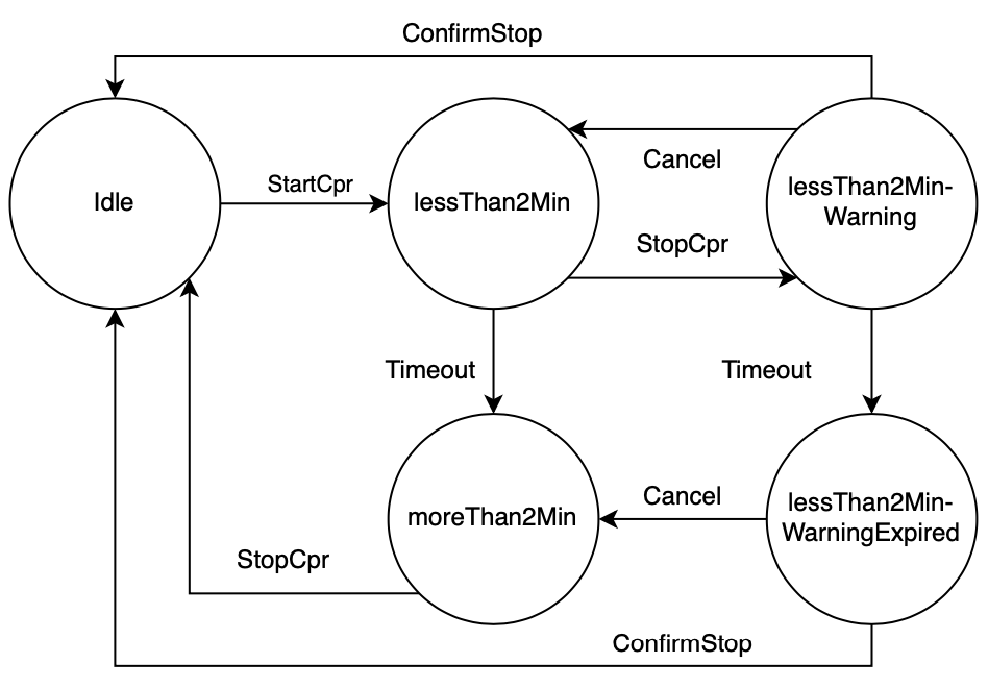
\includegraphics[width=0.55\linewidth]{cpr-machine}
  \caption{CPR Machine}
  \label{fig:cpr-machine}
\end{subfigure}%
\hfill\newline\hfill\newline\hfill
\begin{subfigure}{\textwidth}
  \centering
  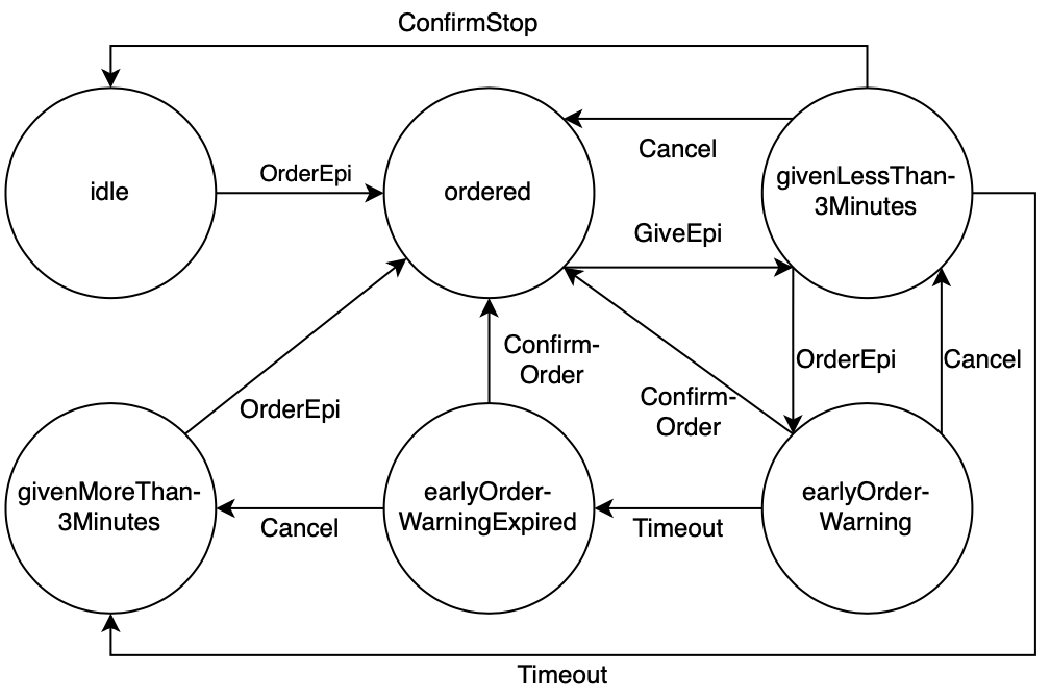
\includegraphics[width=0.55\linewidth]{epi-machine}
  \caption{Epinephrine Machine}
  \label{fig:epi-machine}
\end{subfigure}
\caption{Formal Machine Definitions}
\label{fig:machine-defs}
\end{figure}

At the start of \autoref{sec:kacls-cdss}, we mentioned that
the \emph{frontend} of our \CDSS{} is a simple Javascript-based
application to facilitate user interaction through buttons
and popups. We can now elaborate what we mean by \emph{simple}.
Button presses on the fronend correspond to \emph{events}
that trigger transitions in state machines shown in \autoref{fig:machine-defs}.
For instance, pressing the \say{Start} button under
the CPR part of the tool shown in \autoref{fig:kacls-snapshot} results in a
a \inlinek{StartCPR} event that triggers the corresponding transition in
the machine in \autoref{fig:cpr-machine}.
Similarly, certain machine states result in events being dispatched
to the frontend that cause popups or messages to be displayed
on associated parts of the screen. Thus, the frontend itself contains
no medical logic.

\subsection{$\KACLS$ backend}\label{sec:kacls-backend}

As described at the start of \autoref{sec:kacls-cdss},
the backend receives events from the frontend, processes them and
dispatches the results back to the frontend.
In \autoref{sec:execution-specific-details}, we described the
process of details required for execution by expressing
the \BPG{} using communicating state machines. For a functioning
backend through, we need to translate the abstract state machines
into an executable medium. We do this by encoding the
state machines in a $\K$ definition. Before we describing the
encoding, we describe some additional challenges that we need
to address in order to use $\K$ as a \CDSS{} backend.

\subsubsection{Additional Challenges}

\paragraph{Asynchronous External Communication:}
Communication with external process in \K{} is facilitated
through the use of built-in I/O support. \K has built-in
functions for many operations that map directly to their
POSIX counterparts \cite{KFrameworkIOUrl}. However,
execution in $\K$ is single-threaded. Thus, to make \K{}
behave as an HTTP \cite{HTTPUrl} server that accept messages and respond asynchronously,
we need to write additional C++ initialization code and link it against
\K's LLVM backend \cite{KFrameworkBackendsUrl}.

\paragraph{Handling Timers:}
The \ALS{} workflows shown in \autoref{fig:acls-algorithm} require
tasks being performed periodically. For instance, the algorithm
calls for continuous CPR administration for two minutes
between checking rhythm and performing defibrillation if needed.
Similarly drugs like epinephrine must be administered every three minutes.
\K{} does not support setting timers that can interrupt the \K{} process
on expiration. Thus, we rely on external \say{timers} that, instead
of interrupting the \K{} process, place a \inlinek{timeout} event
at the head of the \inlinek{<inputBuffer>} cell on expiration, which
trigger corresponding transitions in state machines. For example,
consider the CPR machine in \autoref{fig:cpr-machine}. When
\CPR{} is started through the press of a button on the frontend,
an external two minute timer is set, and the machine
transition from state \inlinek{idle} to \inlinek{lessThan2Min}.
When the timer expires, the external timer sends a \inlinek{Timeout}
event to the \K{}, makes the \CPR{} machine to transition from
state \inlinek{lessThan2Min} to \inlinek{morethan2Min}.

\subsubsection{$\KACLS{}$ Backend}
Recall from \autoref{sec:semantics-in-k} that in $\K$ computation
is described via rewrite \emph{rules} that operate over a \emph{configuration}
that organizes data in labeled and potentially nested units called cells.
\autoref{lst:initial-configuration} shows the initial configuration for
the definition $\K$ of our state machines-based representation.
Note that unlike a typical $\K{}$ definition, the initial \inlinek{configuration}
does not have a \inlinek{<k>} cell containing a \inlinek{$PGM} variable
replaced by the program \AST{} at runtime, as the $\K$ definition is the
program itself.

\begin{lstlisting}[float=ht,
  frame=single,
  style=ksty,
  language=k,
  numbers=left,
  numbersep=5pt,
  caption={Initial Configuration},
  label={lst:initial-configuration},
  xleftmargin=3ex
]
    configuration
        <machines>                                @\label{lstline:machines-cell-start}@
            <machine multiplicity="*" type="Set"> @\label{lstline:machine-cell-start}@
                <id>    .K   </id>
                <state> .K   </state>
                <store> .Map </store>
            </machine>                           @\label{lstline:machine-cell-end}@
        </machines>                              @\label{lstline:machines-cell-end}@
        <inputBuffer>  .JSONs </inputBuffer>     @\label{lstline:input-buffer-cell}@
        <outputBuffer> .JSONs </outputBuffer>    @\label{lstline:output-buffer-cell}@
\end{lstlisting}

Lines \ref{lstline:machines-cell-start}-\ref{lstline:machines-cell-end} declare
a cell \inlinek{<machines>} that will be used to multiple
\inlinek{<machine> ... </machine>} cells, declared between Lines
\ref{lstline:machine-cell-start} and \ref{lstline:machine-cell-end}, where
each cell stores all data related to a particular state machine. The
\inlinek{<id>} and \inlinek{<state>} cells store the machine's name and
active state respectively. The \inlinek{<store>} cell
is a map used to store any additional data. Note the following:
\begin{enumerate}[label=(\roman*)]
  \item The \inlinek{<machine>} cell is declared with an attribute
    \inlinek{multiplicity=*}, signifying that the configuration can contain
    multiple instances of such cells that are added or removed dynamically
    during execution. At the start of execution, the configuration has
    zero such cells.
  \item As the number of machines to represent is known and remains constant
    during execution, one might ask why they are not declared as a part of the
    initial configuration itself. We clarify that we deliberate not to do, due
    to reasons we explain shortly.
\end{enumerate}

Lines \ref{lstline:input-buffer-cell} and \ref{lstline:output-buffer-cell}
declare cells \inlinek{<inputBuffer>} and \inlinek{<outputBuffer>} respectively
that hold comma-separated lists of
JSON objects. As their name suggested, they are used as buffer to communicate with
the frontend. Incoming events from the
frontend are placed at the end of the \inlinek{<inputBuffer>} and outgoing
events intended for the frontend are consumed from head of the \inlinek{<outputBuffer>}.

\subsubsection{Initialization}

Initialization involves populating the configuration with the
initial state of each state machine. For instance,
\autoref{lst:cpr-initialization} shows the rule that initializes
the CPR Machine to start in state \inlinek{idle} corresponding to the
entry state of the machine in \autoref{fig:cpr-machine}.

\begin{lstlisting}[float=ht,
  frame=single,
  style=ksty,
  language=k,
  numbers=left,
  numbersep=5pt,
  caption={CPR Initialization},
  label={lst:cpr-initialization},
  xleftmargin=3ex
]
 rule <machines>
       ( .Bag => <machine>                                      @\label{lstline:machine-add-begin}@
                     <id> cprMachine </id>
                     <state> idle </state>
                     <store> "cprRunning" |-> false </store>
                     ...
                  </machine> )                                  @\label{lstline:machine-add-end}@
       ...
      </machines>
      <inputBuffer> "cprMachine.init" , IN => IN </inputBuffer> @\label{lstline:init-inputBuffer}@
\end{lstlisting}
Instead of starting \inlinek{<machines>} cell that is pre-populated with
\inlinek{<machine>} cells from the start, we dynamically initialize
machines once the corresponding frontend component is rendered and ready.
For instance, when the CPR part of the tool from
\autoref{fig:kacls-snapshot} has successfully loaded, it sends a \inlinek{"cprMachine.init"},
which is added to the head of the input buffer.
Lines \ref{lstline:machine-add-begin}-\ref{lstline:machine-add-end} of the rule
introduce a new \inlinek{<machine>} cell with name \inlinek{cprMachine} and initial
state \inlinek{idle}. The \inlinek{.Bag} in $\K$, seen on
\autoref{lstline:init-inputBuffer}, represents the absence of a cell, which
the rule rewrites to a \inlinek{<machine>} cell, resulting in its
addition to the configuration under the \inlinek{<machines>} cell.
On \autoref{lstline:init-inputBuffer}, the $\K$ variable \inlinek{IN} matches any list of
JSON elements. Thus, \inlinek{"cprMachine.init" , IN} matches any list with
\inlinek{"cprMachine.init"} at the head of the list (\inlinek{IN} matches the tail of
the list). When the rule fires, the list is rewritten to
just the tail, resulting in the removal \inlinek{"cprMachine.init"}
event from the \inlinek{<inputBuffer>} cell.

\subsubsection{CPRMachine}

The \textit{CPR Machine} encodes the intended CPR procedure
shown in figure \ref{fig:cpr-machine}. As mentioned earlier, when the user clicks
the \say{Start} button in the CPR pane in figure \ref{fig:kacls-snapshot},
an external two minute timer is started. If the user decides to stop CPR before
two minutes are up, a message is displayed to the user warning him of
deviation from the intended guidelines. If the user stops CPR after
two minutes, no warning message is displayed.
\autoref{lst:cpr-machine-start} shows the rule that
fires when the \say{Start} button in clicked.
The rule does the following:
\begin{enumerate}[label=(\alph*)]
  \item Consumes the \inlinek{"StartCpr"} event from the \inlinek{<inputBuffer>} in
    \autoref{lstline:read-inputBuffer}.
  \item Move the machine from state \inlinek{idle} to state \inlinek{lessThan2Min}
    in \autoref{lstline:idle-lessThan2Min}.
  \item Sends a \inlinek{startTimer} action to the frontend via the
    \inlinek{<outputBuffer>} (encoded as JSON) in
    Lines \autoref{lstline:external-timer-start-begin}-\autoref{lstline:external-timer-start-end},
    which results in the start of a two minute timer in the frontend.
\end{enumerate}
Note how features of $\K$ discussed in \autoref{sec:k-framework}
make the definition \emph{concise} yet \emph{descriptive}. Specifically:
\begin{itemize}
  \item The \emph{configuration abstraction} mechanism enables only parts of the
  configuration that are not used in the rule to be easily ignored.
    The \inlinek{...} (dots) on
    \autoref{lstline:machine-abstraction-dots} contents of cell
    not used in the rule to be safely ignored. Other parts
    of the configuration, such as the \inlinek{<machines>} cell
    and the \inlinek{<outputBuffer>} cell need not be mentioned at all.
  \item Localized rewriting enables the rewrite symbol \inlinek{=>} to
    apply on deeply nested subterms. This enables de-duplication,
    as parts of the term that remain unchanged don't have to be
    specified both on the \LHS{} and \RHS{} of the rewrite. For instance,
    the \inlinek{<store>} cell on \autoref{lstline:store-abstraction-dots}
    contains is a map that holds information about the machine, such as
    execution status. Recall that a map with $n$ key-value pairs is
    depicted in $\K$ as
    \inlinekmath{($k_1$ |- $\ v_1$), ($k_2$ |- $\ v_2$), $\dots\ $, ($k_n$ |- $\
    v_n$)}. Localized rewriting enables us to only rewrite the
    value mapped to key \inlinek{"cprRunning"} from any value to
    to \inlinek{true}, and ignore other parts of the map using \inlinek{...}
    notation.
\end{itemize}
\begin{lstlisting}[float=ht,
  frame=single,
  style=ksty,
  language=k,
  numbers=left,
  numbersep=5pt,
  caption={CPR Machine in \K{}},
  label={lst:cpr-machine-start},
  xleftmargin=3ex
]
  rule <machine>
            <id> cprMachine </id>
            <state> idle => lessThan2Min </state>                    @\label{lstline:idle-lessThan2Min}@
            <store> ( "cprRunning" |-> (_ => true) ) ... </store>    @\label{lstline:store-abstraction-dots}@
            ...                                                      @\label{lstline:machine-abstraction-dots}@
       </machine>
       <inputBuffer> "StartCpr" , IN => IN </inputBuffer>            @\label{lstline:read-inputBuffer}@
       <outputBuffer>                                                @\label{lstline:external-timer-start-begin}@
           OUT => OUT +JSONs jsonResponse( cprMachine
                                         | lessThan2Min
                                         | startTimer( .JSONs ) )
       </outputBuffer>                                               @\label{lstline:external-timer-start-end}@
\end{lstlisting}

\subsubsection{Epinephrine Machine}
\begin{lstlisting}[float=h,
  frame=single,
  style=ksty,
  language=k,
  numbers=left,
  numbersep=5pt,
  caption={Epi Machine in $\K$},
  label={lst:epi-machine-rule},
  xleftmargin=3ex
]
  rule <machine>
        <id> epiMachine </id>
        <state> givenLessThan3Min
            => earlyOrderWarningNotification
        </state>
        <store> .Map => ("tentativeOrder" |-> ORDERED) ... </store>
      </machine>
      <inputBuffer> { "event" : "orderEpi"                              @\label{lstline:input-buffer-json-read-begin}@
                    , "data"  : [ ORDERED:Int ] } , IN
                => IN
      </inputBuffer>                                                    @\label{lstline:input-buffer-json-read-end}@
      <outputBuffer> OUT                                                @\label{lstline:output-buffer-warning-begin}@
        => OUT +JSONs jsonResponse( epiMachine
                                  | earlyOrderWarningNotification
                                  | showEarlyOrderWarning( .JSONs ) )   @\label{lstline:output-buffer-warning-end}@
      </outputBuffer>
\end{lstlisting}

The \textit{Epinephrine Machine} encapsulates instructions for administering
the drug Epinephrine to the patient. The corresponding machine is shown in figure
\ref{fig:epi-machine}.  The user orders the drug using the
\say{Order 1mg} button and can administers it using the \say{Give} button in
Epinephrine pane in figure \ref{fig:kacls-snapshot}. Giving the drug results in the
start of a three minute timer, during which if a new order is placed, a warning
is issued.

\autoref{lst:epi-machine-rule} encodes the transition
$\textssf{givenLessthan3Min} \xrightarrow[]{\textssf{orderEpi}}
\textssf{earlyOrderWarningNotification}$ from \autoref{fig:epi-machine}.
The rule fires when it has been less than three minutes
before the last dose and a fresh order for
Epinephrine is put in (Lines
\ref{lstline:input-buffer-json-read-begin}-\ref{lstline:input-buffer-json-read-end}).
Note that the input event here also has a payload corresponding to the dosage,
depicted by a JSON object with fields \inlinek{"event"} for the event's name
and \inlinek{"data"} for the dosage.
As the guidelines dictate that Epinephrine must be administered
every three minutes, ordering fresh Epinephrine is a deviation from the
guidelines. Thus, an appropriate warning message is presented to the user (Lines
\ref{lstline:output-buffer-warning-begin}-\ref{lstline:output-buffer-warning-end}).

\subsubsection{Encoding Remaining Transitions}
Note that we only show a single rule from the \textit{CPR} and
\textit{Epinephrine} Machines as other rules resemble the ones
shown, and have a one-to-one correspondence to transitions in the
state machines in \autoref{fig:machine-defs}. For instance,
the rule in \autoref{lst:cpr-machine-start} encodes the transition
``$\textssf{idle} \xrightarrow[]{\textssf{StartCpr}} \textssf{lessThan2Min}$'' in the
CPR state machine in \autoref{fig:cpr-machine}. To encode the entire machine,
along with the initialization rule,
we encode every transition $u \xrightarrow[]{\sigma} v$
of machine $\mathcal{M}$ as a rewrite rule of the form shown in
\autoref{lst:general-rewrite}
\begin{lstlisting}[float=h,
  frame=single,
  style=ksty,
  language=k,
  label={lst:general-rewrite},
  caption={Transitions as $\K$-Rules}
]
  <machine>
    <id> @$\mathcal{M}$@ </id>
    <state> @$u$@ => @$v$@ </state>
    ...
    <machine>
  <inputBuffer> @$\sigma$@, IN => IN </inputBuffer>
\end{lstlisting}

\subsubsection{Shock Machine}

We now desribe the \textit{Shock Machine}. Intuitively, this
machine ensures:
\begin{enumerate*}[label=(\alph*)]
  \item shocks are only administered if the rhythm is shockable,
  \item CPR is administered every two minutes, and,
  \item drugs (such as Epinephrine) are periodically administered.
\end{enumerate*}
In case the of deviation appropriate warnings are issued. The \textit{Shock}
machine differs from other machines, as its transitions depend
on the status of the \textit{CPR} machine, as well as the \textit{Shock}
machine.
\begin{lstlisting}[
  frame=single,
  style=ksty,
  language=k,
  numbers=left,
  numbersep=5pt,
  caption={Shock Machine in $\K$},
  label={lst:shock-machine},
  xleftmargin=3ex
]
    rule <machine>
            <id> shockMachine </id>
            <state>
              shockableRhythm => checkRhythm
            </state> ...
          </machine>
          <machine>
            <id> cprMachine </id>
            <store> ( "cprRunning" |-> false ) ... </store> ...
          </machine>
          <machine>
            <id> epiMachine </id>
            <store> ( "epiGiven" |-> true ) ... </store> ...
          </machine>
          <inputBuffer> "administerShock" , IN => IN </inputBuffer>
          <outputBuffer> OUT
          => OUT +JSONs jsonResponse( shockMachine
                                    | checkRhythm
                                    | confirmShock("CPR for
                                                    2 Minutes" ) )
          </outputBuffer>
\end{lstlisting}
The rule abovfires when the rhythm is \textit{shockable}, and the user
wants to administer a shock. Additionally, CPR hasn't been administered (line 9), but
Epinephrine has been administered (line 13). In such a situation, a suggestion to
administer CPR for two minutes is displayed to the user (lines 19-20). We draw
the user's attention to the \textit{succinctness} and \textit{simplicity}
of the rule. Despite expressing the interaction between three different machines,
$\K$'s configuration abstraction mechanism ensures that only relevant parts of
each machine are mentioned, making the transition \textit{comprehensible}.

